\documentclass[uplatex,dvipdfmx,a4paper,twocolumn,base=11pt,jbase=11pt,ja=standard]{bxjsarticle}  % 環境に合わせて変更してください

\usepackage{ipsj}
\usepackage{color}

%追加パッケージ
\usepackage{enumerate}
\usepackage{url}
\usepackage[dvipdfmx]{graphicx}
%\usepackage{caption}

\newcommand{\todo}[1]{\colorbox{yellow}{{\bf TODO}:}{\color{red} {\textbf{[#1]}}}}

\title{発生頻度の少ないコーディング規約違反データ統合による\\検出精度向上への試み}{Toward improving detection accuracy by integrating occasional coding convention violations datasets}
\author{和歌山大学}{亀岡 令}{Ryo Kameoka, Wakayama University}
\author{和歌山大学}{伊原 彰紀}{Akinori Ihara, Wakayama University}
\author{和歌山大学}{南 雄太}{Yuta Minami, Wakayama University}
\author{和歌山大学}{大森 楓己}{Fuki Omori, Wakayama University}

\begin{document}
\maketitle

%================
%1
\section{はじめに}
%================
%hogehoge(背景,動機とか)
ソフトウェアを共同開発するプロジェクトでは,コーディング規約を遵守する可読性の高いソースコードの実装が期待される.具体的には,PythonのPEP8やJavaのCode Conventions for the Java Programming Languageなど,各言語が標準的な規約を公開している.コーディング規約はプロジェクト開発のような複数人でコードを書く際に,可読性や保守性を高めるために定められた記法や,ソースコードの特徴量についての規定のことである.多くのプロジェクトでは静的解析ツールを用いることで規約を違反するソースコードの検出を自動化している.しかし,静的解析ツールが検出する違反は膨大であるため,優先的に修正すべき違反の選択が余儀なくされる.

%開発者は保守管理の観点から,コーディング規約を遵守することによって可読性の高いコードを書くことが求められる.コーディング規約とは,ソースコードを記述する際に,保守性や可読性を高めるためにインデントや括弧などの記法を定めたものである.コーディング規約の例として,PythonのPEP8やJavaのCode Conventions for the Java Programming Languageなどがある.ただし,開発者が自らこれらの規約に違反しているコード断片を特定し,修正を行うことは時間的コストを要するため,静的解析ツールツールが用いられる.

従来研究では,機械学習を用いて優先的に修正すべき規約違反を推薦する手法を提案している~\cite{article1}.しかし,一部の規約は発生頻度が低く,修正率や発生率が低い.このような規約は,推薦精度の低下に影響する.特に,新規プロジェクトでは過去に発生した違反修正履歴を持たないため,規約違反の推薦におけるコールドスタート問題の解決は容易でない.


%静的解析ツールは,ツールによって定義されたルールによって該当するすべてのコーディング規約違反を検出することができる.これによってプログラム中のコーディング規約違反が大量に発見されることが多い.だが,開発者がここで発見された規約違反コードをすべて修正することは無い.従来研究では,機械学習を用いて静的解析ツールによって発見された規約違反が修正されたかを学習し,優先して修正すべき規約違反の検出を行っている~\cite{article1}.しかし,規約違反の種類ごとの分布には偏りがあるため,違反頻度の低い規約は機械学習において,予測精度は学習データセットの大きさ,正例不例の割合などに依存する問題が起こる.

%===============
本研究では,優先的に修正する規約違反コード断片の推薦におけるコールドスタート問題の解決に向けて,他のプロジェクトにおける違反修正履歴を用いて推薦モデルを構築する.さらに,発生頻度や修正率が低い規約違反の予測も実現するために,連合学習によってモデルを構築する.連合学習は,学習データから得られたモデルに加えて,別の学習データから得られたモデルも利用してモデルを構築するため,修正率が低いような規約に対しても,他プロジェクトの学習データを用いることで予測を可能にする.本研究では,プログラムの編集履歴からソースコード本体や変更に関する特徴量を計測し,特徴量を学習データとして連合学習の代表的な手法であるFedAvgを用いてモデルを構築する.
% \todo{検証のことまでここに書くか結果などの分量によって要検討.}


%本研究では,連合学習を用いて学習することで,予測精度の向上させることを目的とする.連合学習は,学習データから得られたモデルに加えて,別の学習データから得られたモデルも利用してモデルを構築するため,それぞれの学習データセットの特徴を考慮することができる.具体的には,プログラムの編集履歴を特徴量とし,違反が修正された編集の特徴をもとにし,連合学習によって構築されたモデルを利用することで,規約違反が修正させるかを予測する.
%================
%2
\section{分析}
%================

\subsection{モデル構築方法}
モデル構築には,従来研究で使用された9件の説明変数に,変更行数や複雑度などソースコードの特徴量を加えた44個の特徴量を用いて,FedAvgを用いた連合学習によりモデルを構築する~\cite{article2}.目的変数は,特定のコミットにおいて編集されたファイルに含まれる規約違反の修正有無の2クラス分類に取り組む.本研究で用いた連合学習はリポジトリごとの深層学習によって得られたモデルを集約し加重平均を取り,出力されたモデルをそれぞれの深層学習に配布する.配布されたモデルを用いて個々のノードは再度学習を行う.モデルの構築,得られたモデルの集約,再度学習を繰り返すことで,より精度の高いモデルを得る.本研究では,オープンソースフレームワークのOpenFLを用いて実装する.その際,最適化アルゴリズムにはAdamを利用し,学習率は0.01に設定した.

% FedAvgにおいて,深層学習のレイヤーは3層で,1,2層目はReLU層であり,3層目にシグモイド関数を用いた出力層となっている.\todo{この3層の説明は必要?}最適化アルゴリズムにはAdamを利用し,学習率は0.01に設定した.

評価実験では,規約違反を修正したコミットが偏っていることがあるため,予測データに正例が極端に含まれていないことを避けるため,コミットの古い順に7割を学習データ,残り3割を予測データとする.



%================
%hogehoge(どんなデータセット使ったか)

%fugofugo(そこからどんなデータをどうやって集めたか)

%2.1の修正版



%================
%2.2
\subsection{ケーススタディ}
本研究では,GitHubで管理される10リポジトリ (transitions, schematics, schema\_salad, python-bugzilla, python-cloudant, pyscard, pynput, OWSLib, howdoi, hickle) を対象とする.これらソフトウェアは全てPythonで実装され,Pylintを使用している.本研究では,それぞれ1,000日間のコミット(中央値で501コミット)を分析対象とする.

%からPythonで実装されておりPylintを用いて開発しているtransitions, schematics, schema\_salad, python-bugzilla, python-cloudant, pyscard, pynput, OWSLib, howdoi, hickleの10リポジトリを対象とする.これらのリポジトリからそれぞれ1,000日間のコミット(中央値で501コミット分)を分析対象とする.



%===============
%FLの説明用図
%===============
%\begin{figure}[t]
%  \centering
%  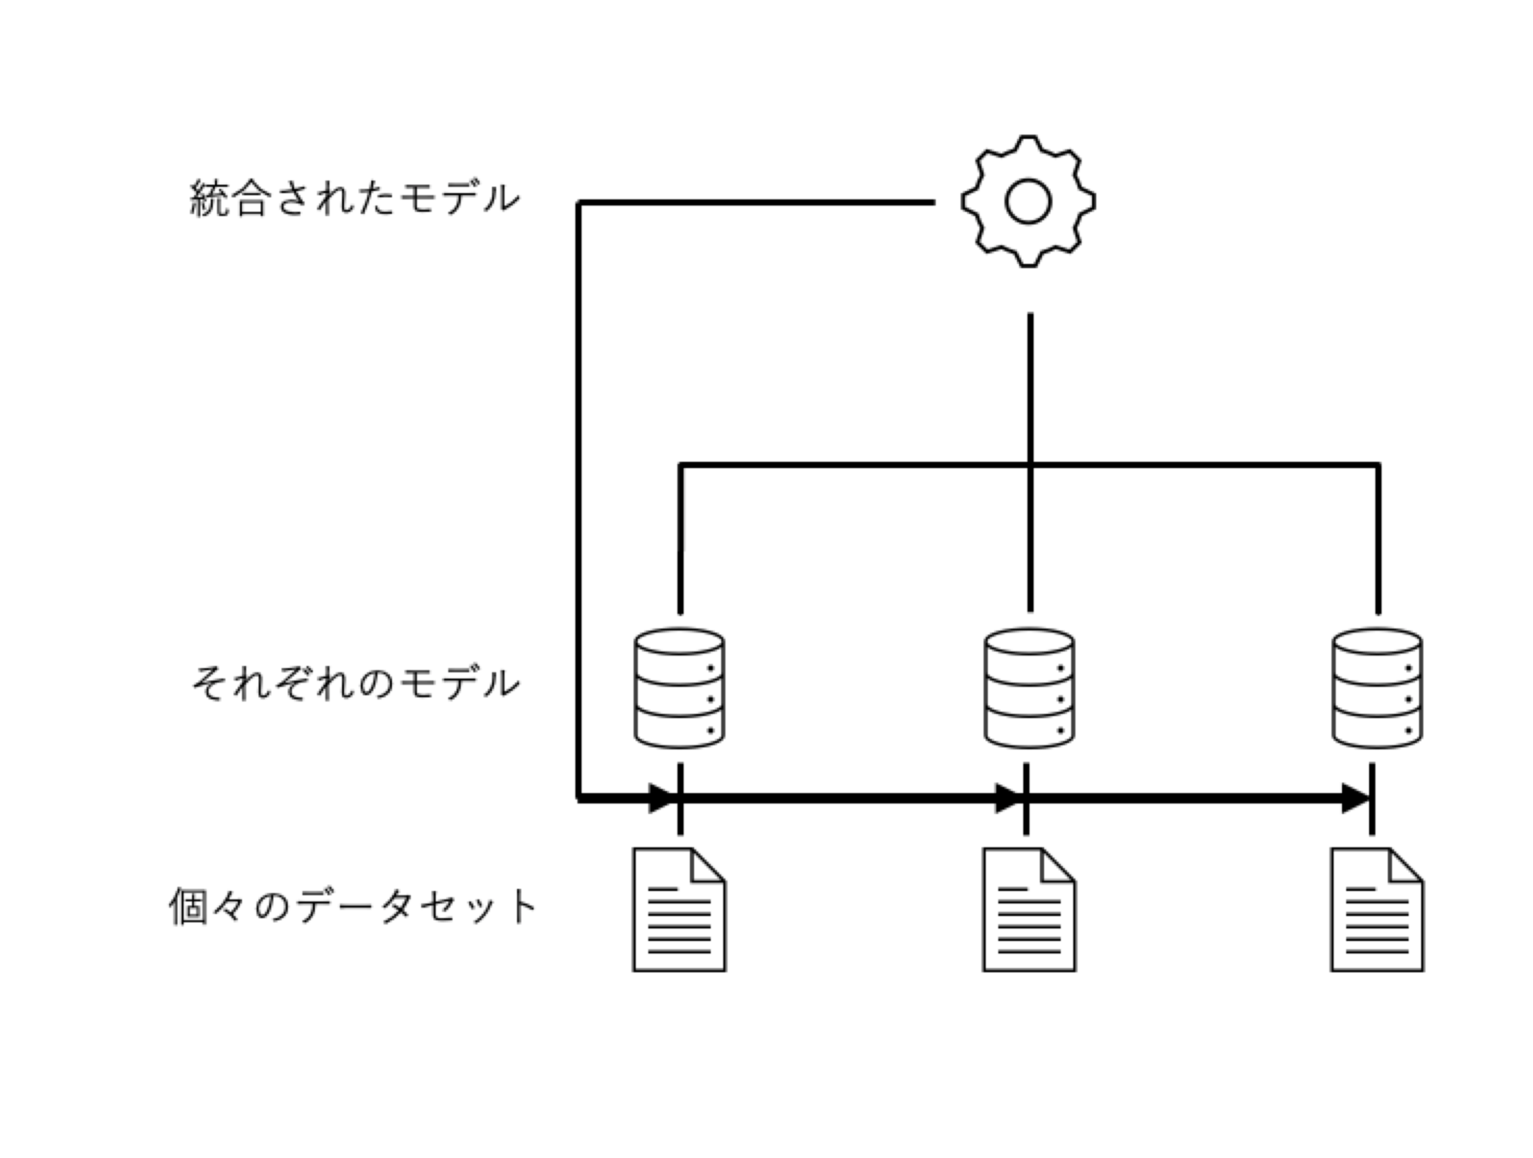
\includegraphics[width=6.5cm]{federated_learning_exp.pdf} 
%  \caption{連合学習}
%  \label{fig:test}
%  \end{figure}

%\begin{figure}[t]
%	\centering
%	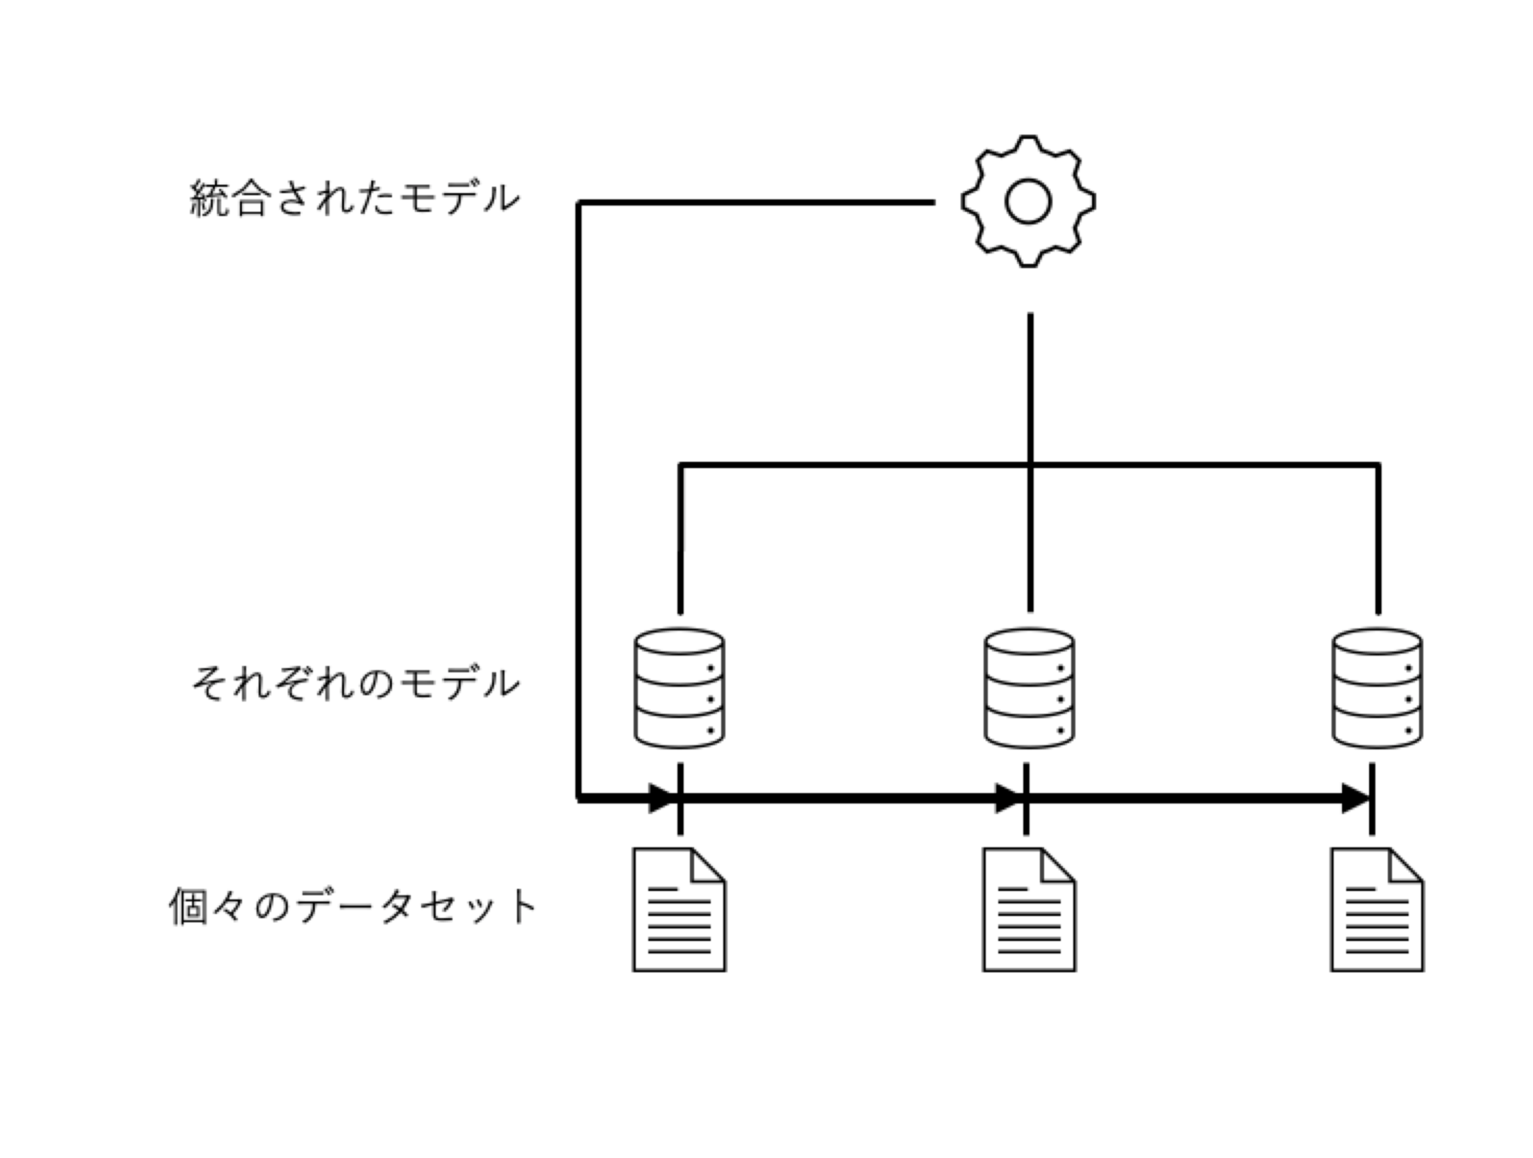
\includegraphics[width=1.0\linewidth]{federated_learning_exp.pdf}
%	\caption{連合学習の概略図}
%	\label{fig:test}
%\end{figure}

%-----------
%\begin{figure}
%\begin{center}
%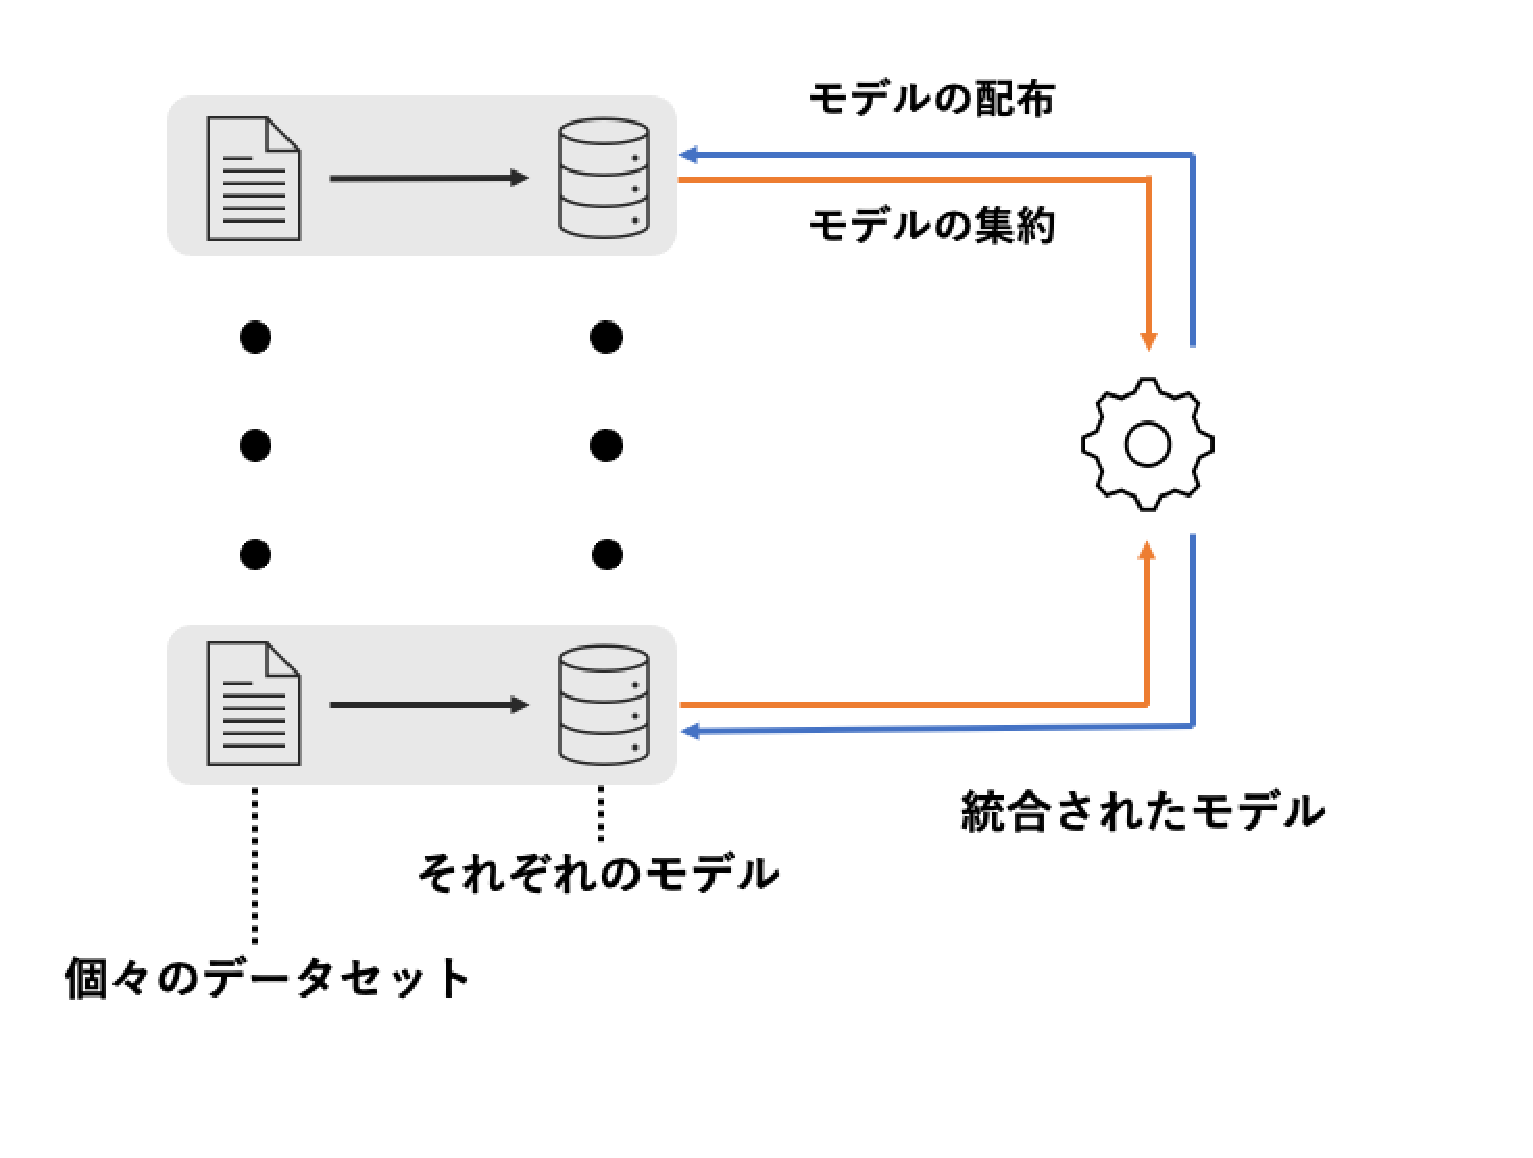
\includegraphics[width=0.9\linewidth]{federated_learning_exp.eps}
%\vspace{-8mm}
%\caption{連合学習の概略図}
%\label{fig:explain}
%\end{center}
%
%\vspace{-7mm}

\begin{figure}
\begin{center}
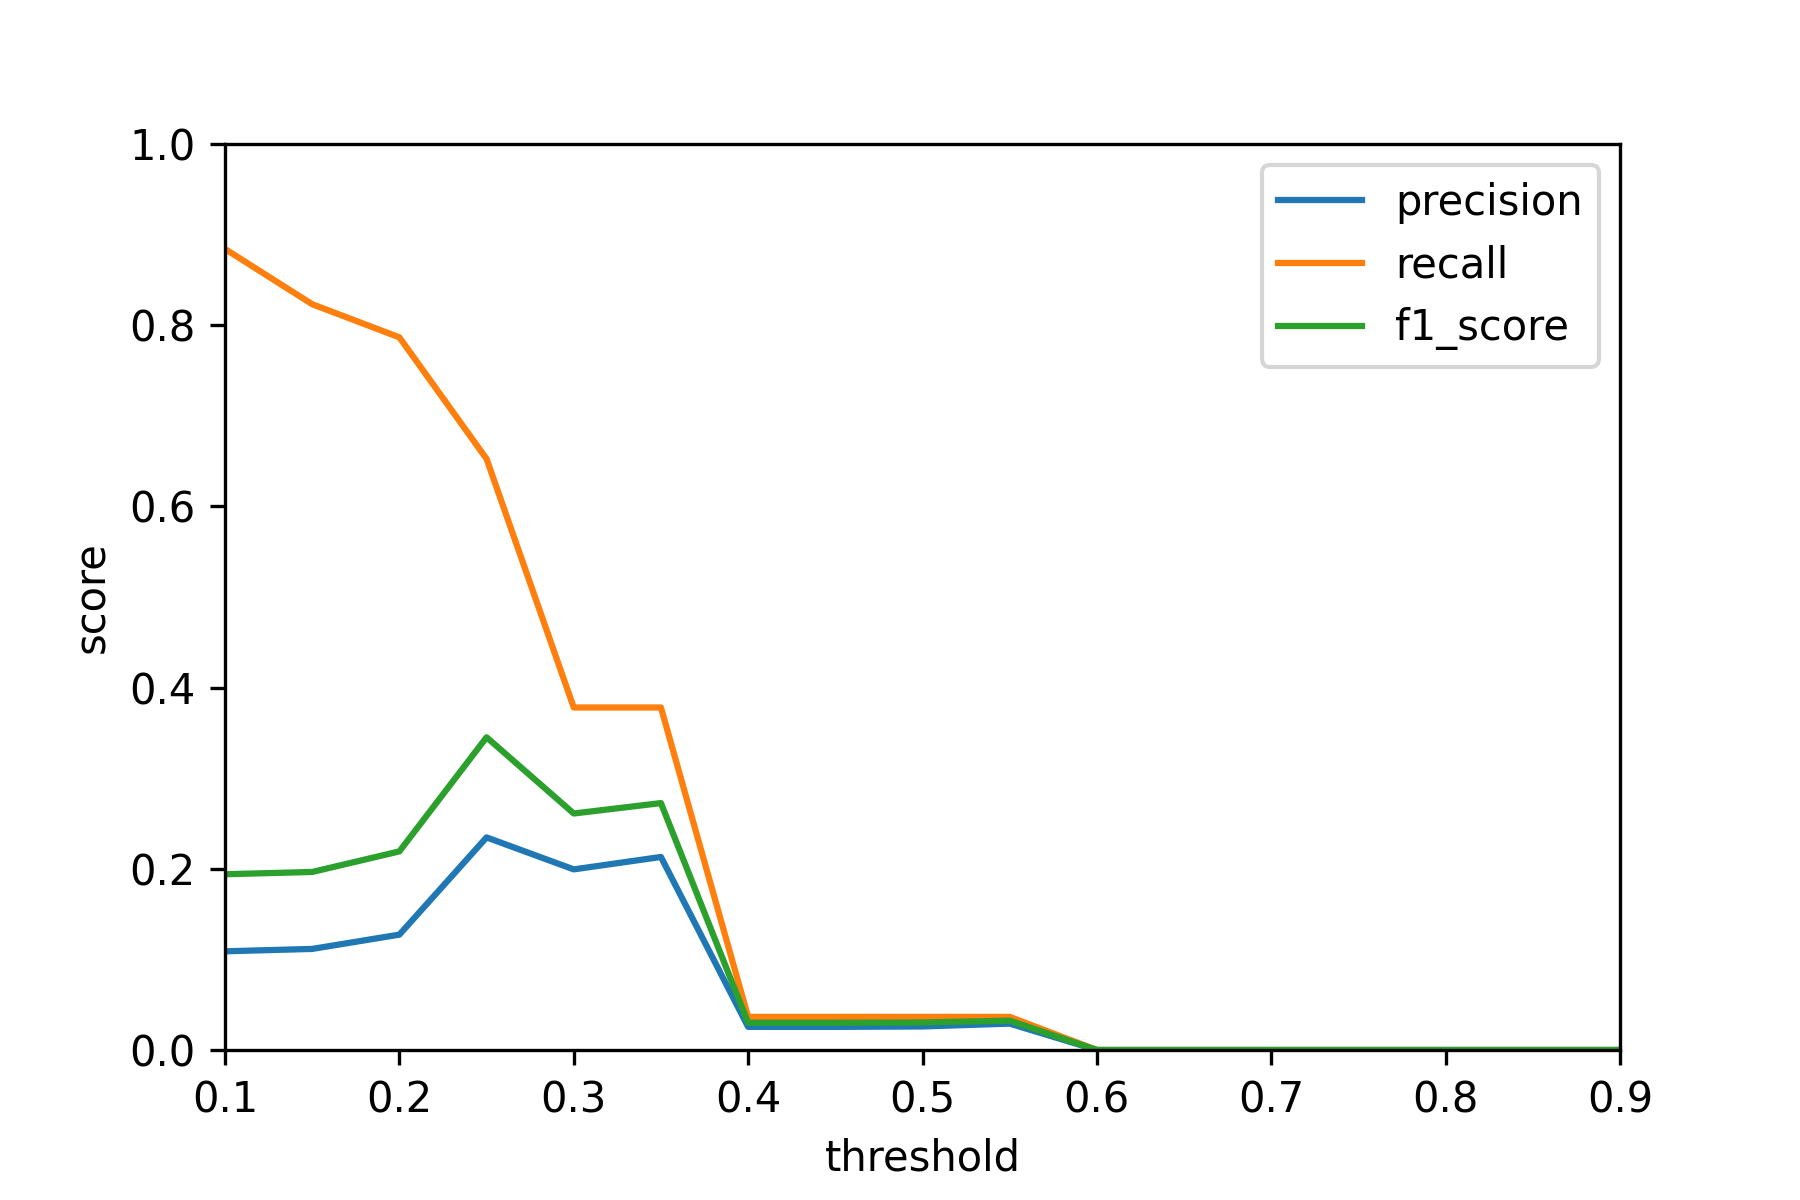
\includegraphics[width=0.9\linewidth]{E0602federated_learning.eps}
\vspace{-3mm}
\caption{連合学習による予測結果}
\label{fig:fed}
\end{center}

\vspace{-8mm}

\begin{center}
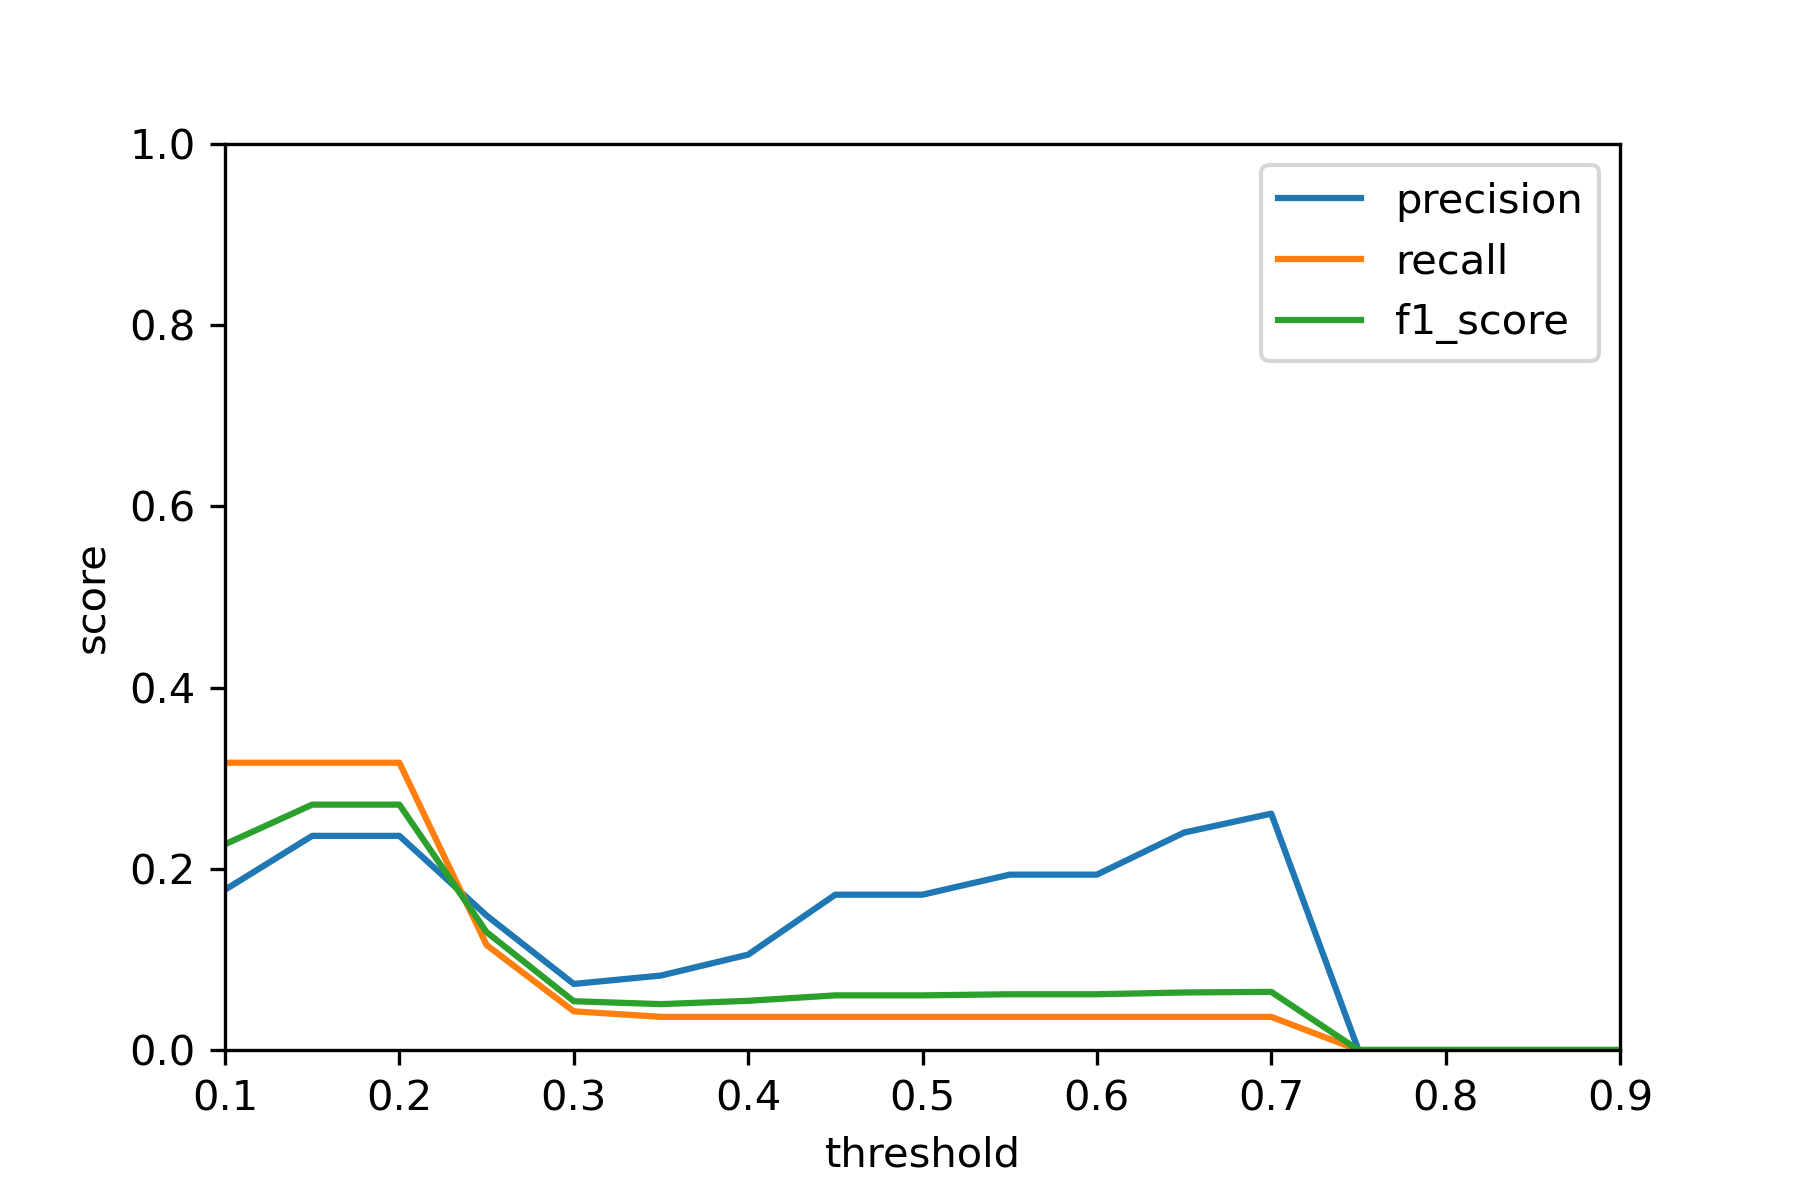
\includegraphics[width=0.9\linewidth]{E0602deep_learning.eps}
\vspace{-3mm}
\caption{深層学習による予測結果}
\label{fig:deep}
\end{center}
\vspace{-12mm}
\end{figure}


%================
%結果の表

% \begin{table}[t]
% \vspace{0mm}
 % \centering
 % \caption{分析結果}
% \label{tab:result3}
  % \scalebox{1.0}{
  % \begin{tabular}{l|r|r|r} \hline
    % & \multicolumn{1}{c|}{適合率} & \multicolumn{1}{c|}{再現率} & \multicolumn{1}{c}{F1値} \\ \hline
    % 連合学習モデル & 0.03 & 0.52 & 0.06 \\ \hline
    % 深層学習モデル & 0.03 & 0.32 & 0.05 \\ \hline
  % \end{tabular}
    % \label{tab:result1}
   % }
% \end{table}

%連合学習(over)
% 正解率: 0.613
% 適合率:  0.034
% 再現率:  0.523
% F1値:  0.063

%連合学習(under)
% 適合率:  0.03799660941991597
% 再現率:  0.28169398907103826
% F1値:  0.06696109631746444

%深層学習(over)
% 適合率:  0.02880505941352306
% 再現率:  0.3185792349726776
% F1値:  0.052833095448469605
%================
%2.4
図~\ref{fig:fed}は,2つのリポジトリ(schematics,transitionsにおいて,修正回数が少ない規約1種類(E0602/undefined-variable)についての修正有無を予測した結果である.横軸は判別閾値を0から1まで変化させたときの適合率,再現率,F1値を示す.図~\ref{fig:deep}は比較対象として,連合学習の際に用いたモデルと同じモデルを利用した深層学習を用いた結果を示す.深層学習に比べ連合学習の方が高い精度で予測しているが,紙面の都合上,検出頻度が低い規約の結果のみ示しているが,修正率が高い規約であっても連合学習の方が精度が高いことを示した.従って,クロスプロジェクトによって規約違反の修正予測は,単純に学習データを結合し深層学習する場合より,効果的に学習を行うことができ,コールドスタート問題の解消への兆候を確認することができた.

% (結論候補1)連合学習を用いたクロスプロジェクトでの規約違反の修正予測は,単純に学習データを結合し,深層学習する場合より効果的に学習を行うことができる.

%連合学習が,深層学習
%
%,が低い場合に連合学習の再現率が高く,深層学習のモデルは閾値に関わらず全体的にすべての値が低いことがわかる.閾値が低い場合にも深層学習では再現率が低いことから,修正予測に必要な重みづけができていないことがわかる.
%
%図~\ref{fig:fed}の結果おいて閾値が0.35の場合に最も適合率,再現率,F1値のバランスが取れていることがわかる.しかし,閾値が0.4以上の場合には,適合率に大きな変化がないが,再現率が下がっている.したがって,連合学習によって規約違反修正の予測に効果がある兆候が確認できるが,モデルとして不十分である.

%どう結果を本文(主張)に繋げるか
%================
%hogehoge(どんな結果が得られたか,図とかを一緒に載せる)

%fugofugo(結果からの考察)
%分析を行った結果次のような結果が得られた.

%--------------------------------表入れるとこ



%================
%3
%\todo{最後に読み直す}
\section{おわりに}

本研究では,静的解析ツールによって検出された規約違反のうち,特に修正回数や発生回数が低いものについて,連合学習によって修正されるかの予測を試みた.今後の方針として,データセットの拡張,違反頻度の低い規約違反への重み付けなどを用いて予測精度の高いモデルの構築を目指す.
%================

%hogehoge(今回の研究のまとめとか)

%fugofugo(今回研究から得られたことを踏まえて今後どう発展させていくか)

%42(どんな研究をしていくつもりなのか的な)
%今回の研究のから hogehoge-fugofugoである.

%\begin{figure}[h]
%  \centering
%  \includepraphics[width=6.5cm]{example.png}
%  \caption{図のキャプション}
%\end{figure}


%================
\section*{謝辞}
本研究は和歌山大学「萌芽的個別研究支援」の助成を受けたものです.
%================


\begin{thebibliography}{1}
    \bibitem{article1} J. R. Ruthruff, J. Penix, J. D. Morgenthaler, S. Elbaum, and G. Rothermel: Predicting Accurate and Actionable Static Analysis Warnings: An Experimental Approach: Proc. of the Inter. Conf. on Software engineering (ICSE), pp. 341-350, 2008.
    \bibitem{article2} B. McMahan, E. Moore, D. Ramage, S. Hampson, B. A. y Arcas: Communication-Efficient Learning of Deep Networks from Decentralized Data: Proc. of the Inter. Conf. on Artificial Intelligence and Statistics (PMLR), pp. 1273-1282, 2017.
\end{thebibliography}




\bibliographystyle{ipsjunsrt}
%\bibliography{bibfile}

\end{document}
